\section{Background reading}
\subsection{Introduction}
Creating the algorithm for lane detection involves two major steps: collecting and marking
data and creating the algorithm itself. 

Lack of finance makes me find a way to mark up the dataset in an autonomous way. To do this
I will try non-ML and some unsupervised learning methods of marking.
The second step is creating the algorithm itself. After the CNN revolution that 
happened in CV more than 10 years ago, when AlexNet was presented\cite{alexnet}, many different approaches and
architectures were created, most of which can be used almost on any hardware for almost any task. 
In this review, my goal is to choose a few of them, test and find one that suits my task best.

\subsection{Data preprocessing}
\subsubsection{Introduction}
All ML projects start with collecting a dataset. So I followed the same procedure. 

The dataset was collected using Duckiebot. A small server was created 
using GoLang to receive images from the bot's camera. After that a few 
different approaches were used to mark it up. All approaches had some disadvantages that will
be listed below:

\subsubsection{Non-ML approach}
\begin{figure}[h]
    \begin{center}
        
    
    \subfloat[raw image]{\label{fig:lena-raw}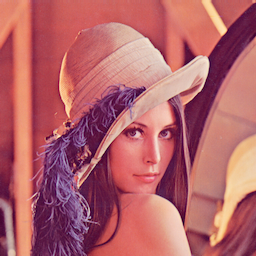
\includegraphics[scale=0.32]{src/BackgroundReading/assets/Lenna.png}}
    \subfloat[brightness map]{\label{fig:lena-brightness}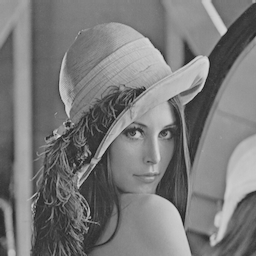
\includegraphics[scale=0.32]{src/BackgroundReading/assets/Lenna brightness.png}}
    \subfloat[energy map]{\label{fig:lena-energy}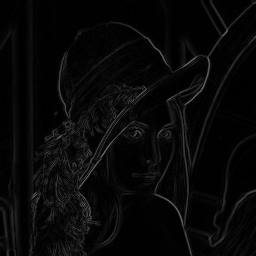
\includegraphics[scale=0.32]{src/BackgroundReading/assets/Lenna energy.png} }
    \subfloat[scaled energy map]{\label{fig:lena-scaled-energy}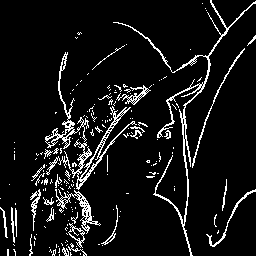
\includegraphics[scale=0.32]{src/BackgroundReading/assets/Lenna energy_with contrast.png}}
    \\
    \subfloat[raw image]{\label{fig:road-raw}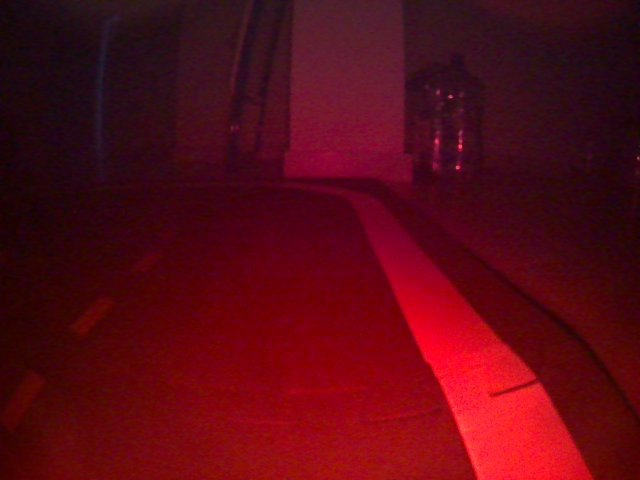
\includegraphics[scale=0.1295]{src/BackgroundReading/assets/615.png}}
    \subfloat[brightness map]{\label{fig:road-brightness}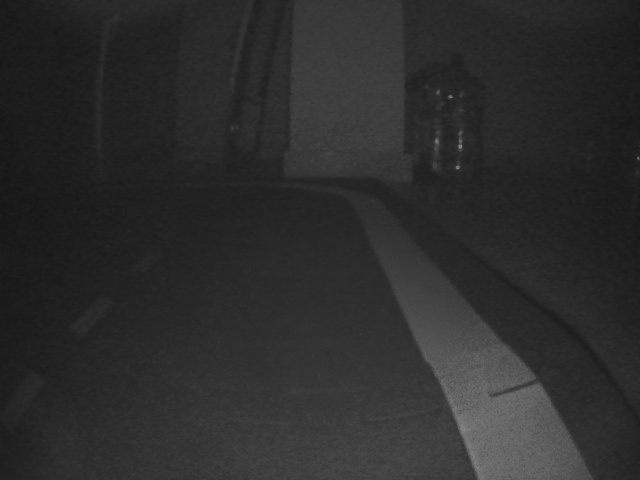
\includegraphics[scale=0.1295]{src/BackgroundReading/assets/615 brightness.png}}
    \subfloat[energy map]{\label{fig:road-energy}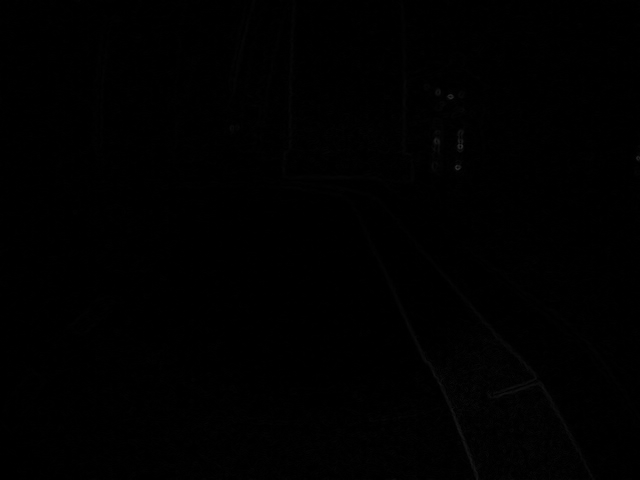
\includegraphics[scale=0.1295]{src/BackgroundReading/assets/615 energy.png} }
    \subfloat[scaled energy map]{\label{fig:road-scaled-energy}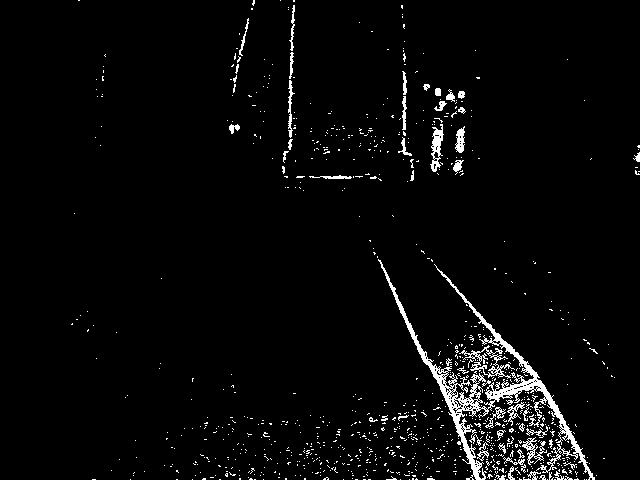
\includegraphics[scale=0.1295]{src/BackgroundReading/assets/615 energy_with contrast.png}}
    \end{center}

    \caption{Results of each step for high contrast and low contrast image}
\end{figure}
The first idea was to use a non-ML approach based on ``energy``.~\cite{seamcarving} 

The main ideas of this approach are:
\begin{enumerate}
    \item Convert RGB pixels to brightness
    \item Use discrete derivatives of brightness to compute energy
\end{enumerate}
\begin{enumerate}
    \item \textbf{Brightness}\\
To convert RGB image to brightness map it was decided to use Y 
component of YCbCr color space, because this component shows the 
brightness. To convert RGB image to YCbCr we need to use simple 
operation~\cite{YCbCr}:
\[\begin{pmatrix}
    Y' \\
    Cb \\
    Cr
\end{pmatrix} = 
\begin{pmatrix}
    0.257 & 0.504 & 0.098 \\
    -0.148 & -0.291 & 0.439 \\
    0.439 & -0.368 & -0.071
\end{pmatrix} \cdot
\begin{pmatrix}
    R \\
    G \\
    B
\end{pmatrix} + 
\begin{pmatrix}
    16 \\
    128 \\
    128
\end{pmatrix}\]
\item \textbf{Energy}
For energy, it was decided to use the formula from 
seam carving paper~\cite{seamcarving}:
\[e_1(I) = |\frac{\partial}{\partial x} I| + |\frac{\partial}{\partial y} I|\]
Where 
\[|\frac{\partial}{\partial x} I_{i,j}| = \frac{I_{i+1,j} - I_{i-1,j}}{2}\]

The intention was to use this algorithm to find a contour of road markup. 
Unfortunately, this approach performs well on high-contrast images, but the project's problem is that images in the dataset 
can and should be low contrast. So this method was abandoned.
\end{enumerate}

\subsubsection{KNN approach}
\begin{figure}[h]
    \begin{center}
    \subfloat[Raw image]{\label{fig:edge-a}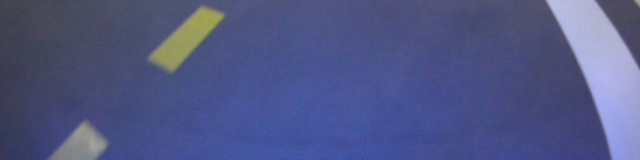
\includegraphics[scale=0.2]{src/BackgroundReading/assets/Raw.png}}
    \subfloat[Middle lane mask]{\label{fig:edge-b}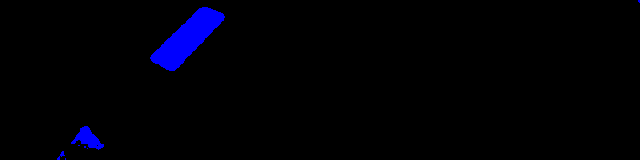
\includegraphics[scale=0.2]{src/BackgroundReading/assets/Middle line.png}}
    \subfloat[Side lane mask]{\label{fig:edge-c}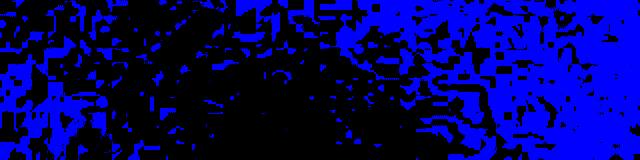
\includegraphics[scale=0.2]{src/BackgroundReading/assets/Side line.png} }
    \subfloat[Road mask]{\label{fig:edge-d}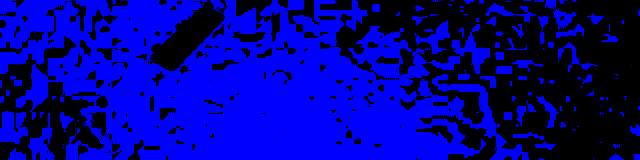
\includegraphics[scale=0.2]{src/BackgroundReading/assets/Road.png}}
    \end{center}
    \caption{Masks provided by KNN algorithm}
\end{figure}
The second thought was about KNN~\cite{knn}. It's powerful, but the computational heavy clustering algorithm can be used in unsupervised learning. 
I tried to use it in two ways:
\begin{enumerate}
    \item Use only color for clustering
    \item Use colors and position of pixels
\end{enumerate}

Both approaches had their advantages and disadvantages, but in the end this method
was rejected, because it couldn't provide good markup even on 
bright images.

\subsubsection{EM algorithm}
\begin{figure}[h]
    \begin{center}
        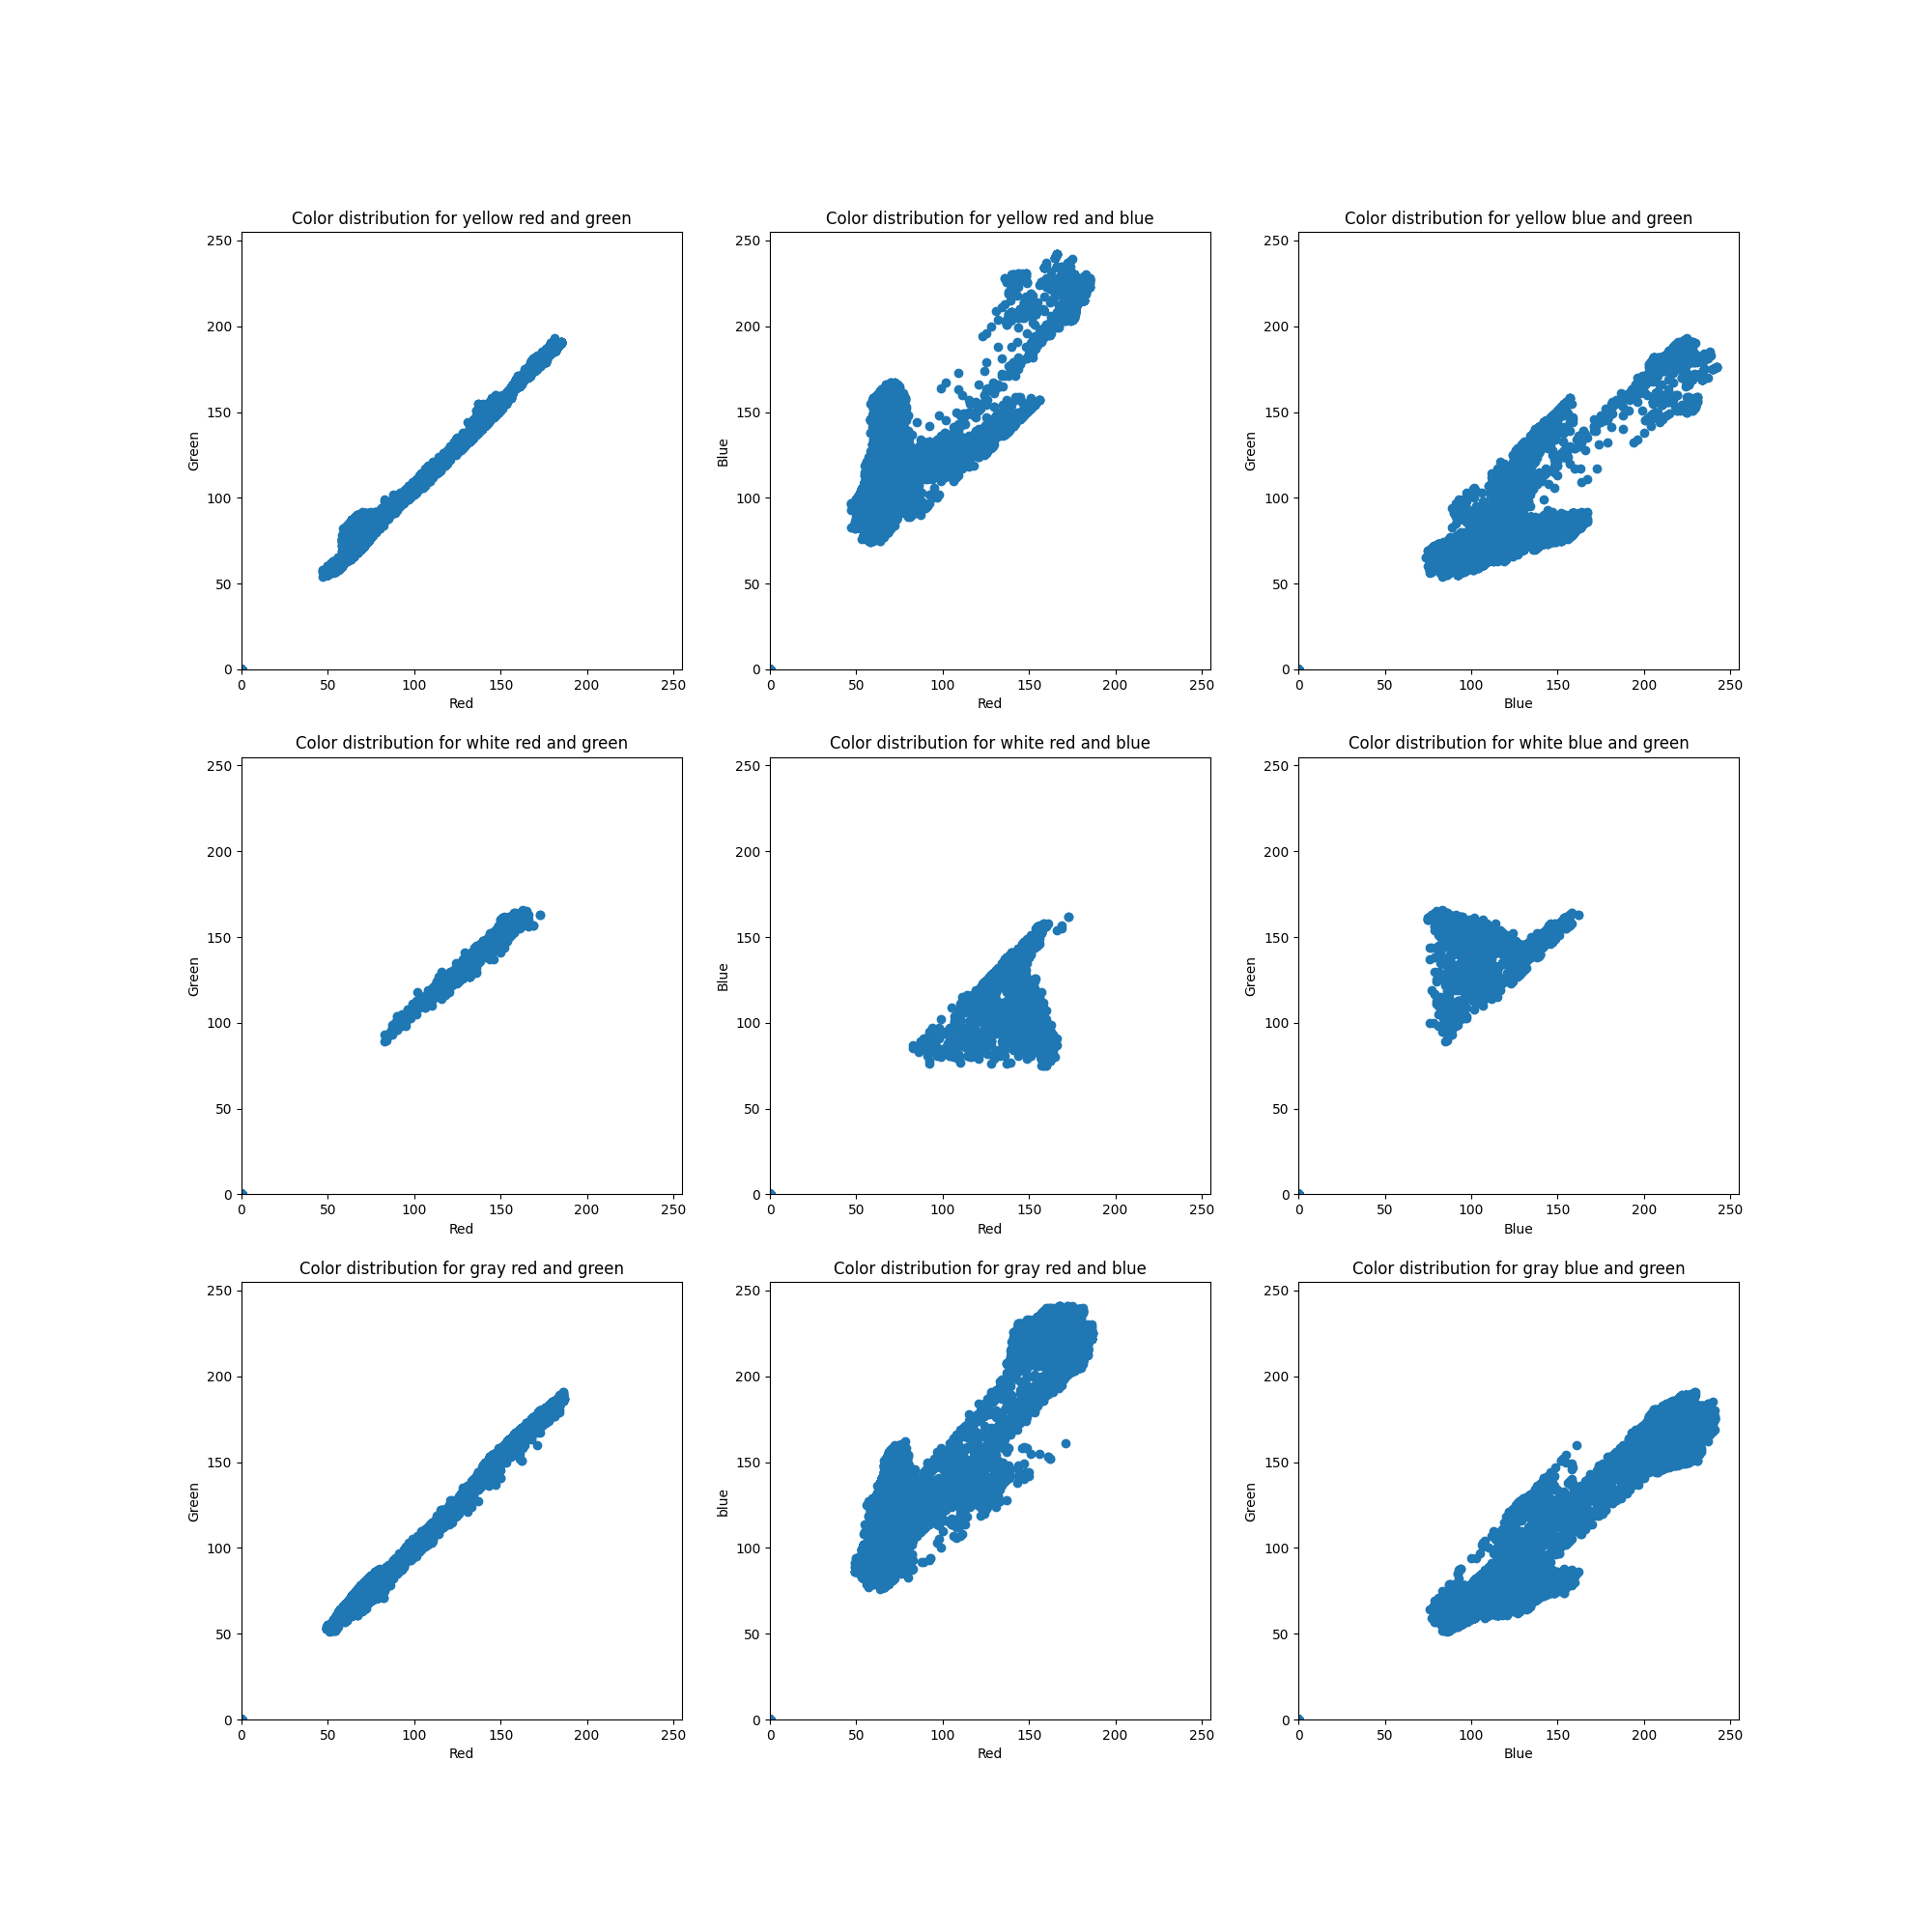
\includegraphics[scale=0.232]{src/BackgroundReading/assets/Distr.png}
    \end{center}
    \caption{Color distribution on images}
\end{figure}

\begin{figure}[h]
    \begin{center}
    \subfloat[Raw image bad sample]{\label{fig:road-raw-bad}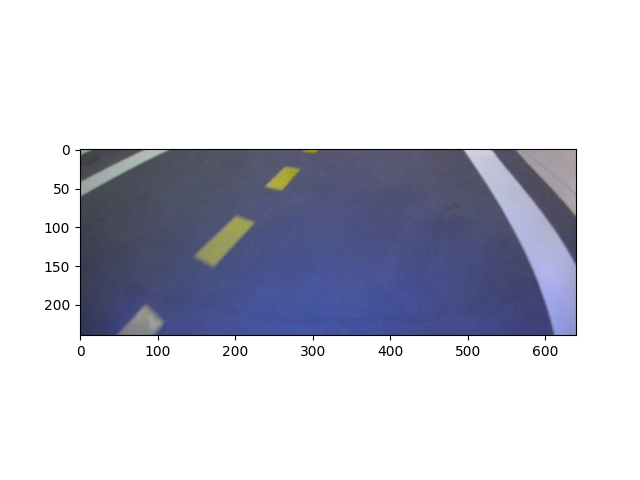
\includegraphics[scale=0.17]{src/BackgroundReading/assets/RawEMBad.png}}
    \subfloat[Mask bad sample]{\label{fig:road-mask-bad}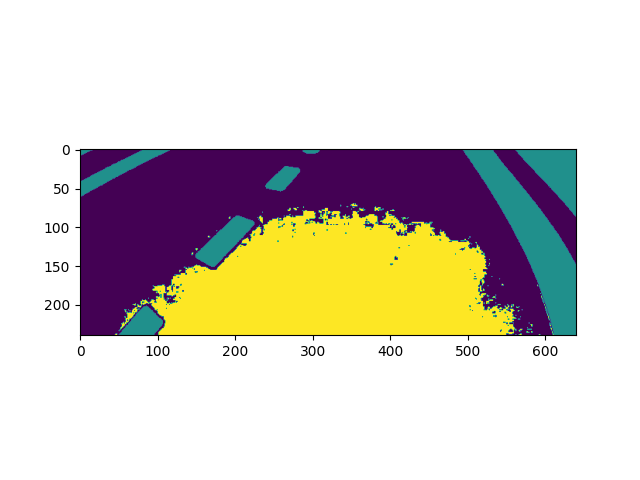
\includegraphics[scale=0.17]{src/BackgroundReading/assets/MaskEMBad.png}}
    \subfloat[Raw image good sample]{\label{fig:road-raw-good}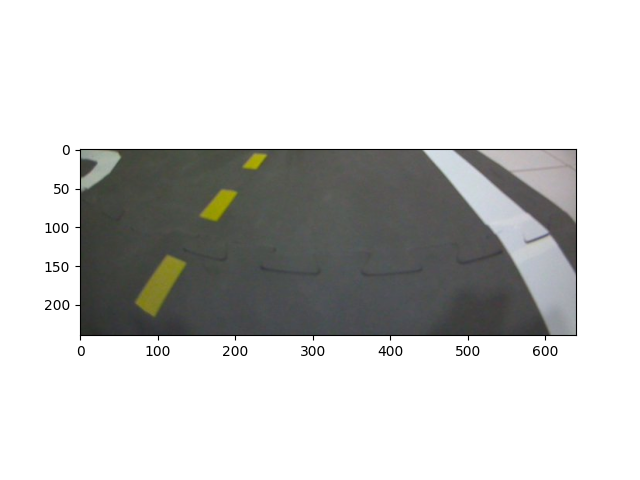
\includegraphics[scale=0.17]{src/BackgroundReading/assets/RawEMGood.png} }
    \subfloat[Mask good sample]{\label{fig:road-mask-good}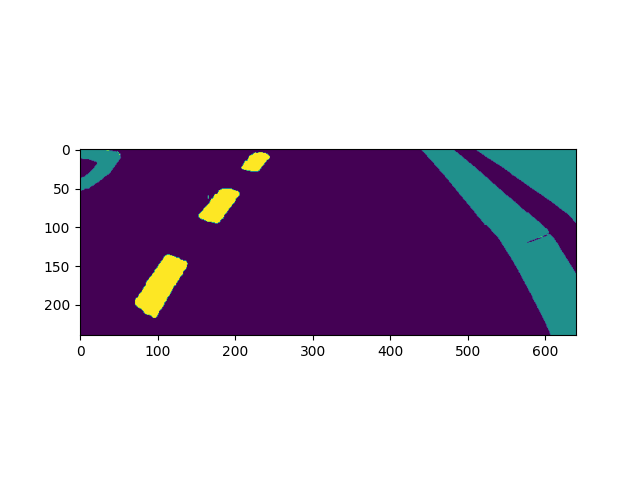
\includegraphics[scale=0.17]{src/BackgroundReading/assets/MaskEMGood.png}}
    \end{center}
    \caption{Masks provided by EM algorithm}
\end{figure}


Last hope was the EM\cite{em1}\cite{em_algo_2} algorithm. The idea of the EM algorithm is to use 
general knowledge about our world to predict something. In my case, I assumed 
that the color distribution of each image is a mixing of a few Gaussians. 

Assumptions:
\begin{enumerate}
    \item Colour distribution is formed by three Gaussians with parameters: 
    \\
    $\{\bar\mu_1, \Sigma_1\}, \{\bar\mu_2, \Sigma_2\}, \{\bar\mu_3, \Sigma_3\}$
    \item Choosing gaussian is made with probabilities: $\{\pi_1, \pi_2, \pi_3\}$
\end{enumerate}

PDF of Normal distribution is
    
    \[\mathcal{N}(\bar x | \mu, \sigma) = \displaystyle \frac{1}{\sigma \sqrt{2\pi}} \cdot e^{\displaystyle-\frac{1}{2}{(\frac{x-\mu}{\sigma})}^2}\]


The idea of the EM algorithm is simple:
\begin{enumerate}
    \item E-step: fix $\bar\theta$ \- parameters of model, find $\mathbb{E}[z]$ \- math expectation of hidden parameters:

    \[\mathbb{E}[z_{n, k}] = \displaystyle \frac{\pi_k\cdot \mathcal{N}(\bar x_n | \bar \mu_k, \Sigma_k)}{\sum\limits_{l=1}^K \pi_l \cdot \mathcal{N}(\bar x_n | \bar \mu_l, \Sigma_l)}\]
    \item M-step: fix $\mathbb{E}$ and maximize likelihood: $\mathbb{E}[\log p(x,z|\bar\theta)] \overset{}{\underset{\bar \theta}{\longrightarrow}} \text{max}$:

    \[\mathbb{E}[\log p(x,z|\bar\theta)] = \sum\limits_k\Big(\sum\limits_n\mathbb{E}[z_{n,k}]\Big) \log \pi_k + \sum\limits_k\sum\limits_n\mathbb{E}[z_{n,k}]\cdot \log p(\bar x_n|\bar\mu_k,\Sigma_k)\]

Also we can notice, that $\sum\limits_n\mathbb{E}[z_{n,k}] = \mathbb{E}[|C_k|]$, where $|C_k|$ is the amount of samples in cluster $C_k$
\end{enumerate}

The results of the EM algorithm were also poor, but a bit better than KNN's ones:

\subsubsection{Result approach}
The final approach is combining energy with EM, 
then using its outputs as inputs to logistic regression\cite{log_regression} with 
data augmentations\cite{augmentations}\cite{synthetic_data}. 

It was decided that this approach should be more useful, because:
\begin{enumerate}
    \item Data augmentations can help with the inefficient of previous approaches, 
    because applying color filters to `clean' images can emulate the light of LEDs 
    of the Duckiebot without loss of accuracy of EM algorithm predictions
    \item The noise of the labels can be compensated by the size of the 
    dataset\cite{big_data_less_noice}
\end{enumerate}

\subsection{Algorithm implementation}
\subsubsection{Introduction}
To implement the algorithm some DL approach will be used. 
There are a few ways to do it:
\begin{itemize}
    \item Fully connected NN to classify the color of pixel\cite{fully_connected} 
    \item MobileNet\cite{mobileNet}
    \item ShuffleNet\cite{shufflenet}
    \item EfficientNet\cite{efficientnet}
    \item Squeeze-and-Excitation Networks\cite{seNet}
\end{itemize}
\subsubsection{Fully connected NN}
This approach will be used as the baseline in terms of accuracy and computational 
speed

This architecture is extremely easy to implement and it is relatively fast.
~\cite{fully_connected} 
The key idea of fully connected NN is MLP (multi-layer perceptron):

If we have input tensor $X\in \mathbb{R}^{n\times 1}$, we can apply linear transformation to it:
$W\cdot X$, where $W \in \mathbb{R}^{k\times n}$, after that we need to add some 
nonlinear activation (ReLU, sigmoid, Tanh, etc) and apply the same block a few more times
As the last activation, we can use softmax for classification or just leave it as it is for regression

\begin{figure}[ht]
    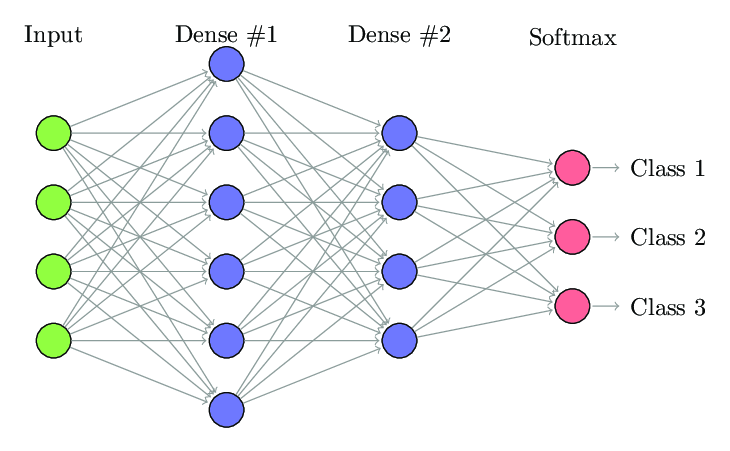
\includegraphics[scale=0.5]{src/BackgroundReading/assets/fully_connected.png}
    \caption{Architecture of fully connected NN with 3 layers}
\end{figure}


But this type of NN isn't so popular in computer vision, because it can't handle 
random-sized images without preprocessing and it struggles with detecting objects 
in different parts of the image. But in the case of this task, it will not be a problem, 
because all images will be the same shape and objects will be in approximately the same spots.
However using a hole image as input tensor will be tough because the image size is $320\times480$ pixels,
so the input tensor will be of size 153600, even if a relatively small hidden layer is used (10000 neurons), 
then one forward pass will be about 23,5 GFLOPs, which is much bigger than CNNs consume.
So this architecture can be used to determine the color of each pixel only independently from others,
this will affect accuracy because such an approach can't determine objects, only colors, which is
good as a baseline, but can't be used in production. 

Determining pixel color will require an input tensor of size 3 (or 5 if positional embeddings are used), 
output tensor will be of size 3 (to show probabilities of belonging pixel to yellow, white or gray color)
and hidden layer can be any size because as a result flops will be: $153600 \cdot( 3 \cdot n + n \cdot 3) = 921600 \cdot n$ FLOPs
if $n$ is less than 20, then such NN can't use more than 18 MFLOPs which is good in comparison with CNN

\subsubsection{MobileNet}
MobileNet Architecture family seems to be a more suitable approach 
as it is relatively fast and has pretty good accuracy on the ImageNet dataset.

Core idea of MobileNet\cite{mobileNet} is splitting standard convolution~\cite{cnn} on two steps:
\begin{itemize}
    \item Using convolution with one channel for each input channel (depthwise convolution)
    \item Use the result of the previous step as input for pointwise convolution 
    (convolution with $1\times 1 \times M$ kernel, where $M$ is amount of input channels) 
    \- this step lets us extract features
\end{itemize}
This approach is fast, because in usual convolution with kernel $D_K\times D_k\times M \times N$ 
(where $D_K$ is kernel size, $M$ \- amount of input channels and $K$ \- amount of output
channels) we need $D_K\cdot D_k\cdot M \cdot N \cdot D_F \cdot D_F$ operations per image 
(we can assume that all images are squared, it is the usual approach in CV). On the other hand in 
MobileNet architecture convolution needs only $D_F\cdot D_F \cdot M \big(D_K \cdot D_K + N)$ 
operations, so we have improved in 
\[ \frac{1}{\frac{1}{N} + \frac{1}{D_K^2}}\] 
Assuming that the usual kernel has size $3\times 3$ it is a significant boost.

Also, this approach reduces memory usage, because each convolutional layer needs
only $M \cdot D_K\cdot D_K + N\cdot M$ parameters, while classical convolutional layer
with the same input hyperparameters needs $M \cdot D_K\cdot D_K \cdot N$

\subsubsection{ShuffleNet}

This model develops ideas of MobileNet (even if it is not fully represented in paper, however, it's obvious).

Authors of ShuffleNet propose to use group pointwise convolution (GPC) instead of 
classical pointwise convolution\cite{shufflenet}. 

The idea of GPC is relatively simple: instead of performing this operation:
$I * K$ (where $*$ is convolution, $I$ is tensor with shape $H\times W \times C \times M$ 
and $K$ pointwise convolution kernel with shape $1\times 1 \times C \times M$, 
$C$ \- amount of input channels, $M$ \- amount of output channels), which
takes $W\cdot H \cdot C \cdot M$ MFLOPs (floating point multiplication-adds), we 
can use this operation:
\[\overset{g-1}{\underset{i=0}{CONCAT}}(I_{[i\cdot g : (i+1)\cdot g]}* K_i)\] 
where $I_{[a:b]}$ \- tnesor which consists of $a$'th till $b$'th channels of tensor $I$. 
Such an approach requires in $g$ times fewer MFLOPs, but we have to face another problem:
output channels, which were produced by one group of input channels `do not know' anything about 
other input channels. To fix this authors of ShuffleNet propose a shuffle layer, which
can be used in the bottleneck block (Figure~\ref{ShuffleNet architecture}).
\begin{figure*}[ht]
    \begin{center}
        \subfloat[ShuffleNet Bottleneck block]{\label{fig:bottle-neck}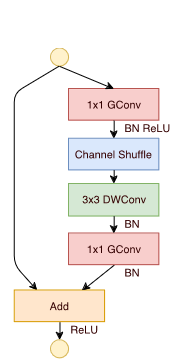
\includegraphics[scale=0.5]{src/BackgroundReading/assets/bottleneck.png}}
        \subfloat[Shuffle layer]{\label{fig:shuffle_layer}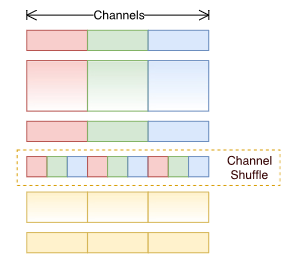
\includegraphics[scale=0.5]{src/BackgroundReading/assets/shuffle_layer.png}}
    \end{center}
    \caption{ShuffleNet architecture}\label{ShuffleNet architecture}
\end{figure*}

If we count MFLOPs of bottleneck block in ShuffleNet and MobileNet 
(we can use its ideas to construct bottleneck block), we will get such results:
\begin{enumerate}
    \item ShuffleNet: $W\cdot H \cdot (\frac{2\cdot C \cdot M}{g} + 9M)$
    \item MobileNet: $W\cdot H \cdot (2 \cdot C \cdot M + 9M)$
\end{enumerate}
As you can see we have a small gain, but we lose some accuracy, even in the article authors
provide us with data, that shows that ShuffleNet isn't always better than MobileNet,
so I will try to implement both of them to find the best one.

\subsubsection{EfficientNet}
EfficientNet also seems to be a good model to try\cite{efficientnet}. 

It uses MobileNetV2\cite{mobile_netv2} bottleneck as main building blocks and this type of architecture
is easy to scale. Moreover base model EfficientNet-B0 has fewer MFLOPs in comparison 
with MobileNet (390 MFLOPs vs 569 MFLOPs), but has a bit more parameters. However, 
the Duckiebot has 4GB RAM so it can handle up to 1 billion parameters, which is much 
bigger than 5 million of EfficientNet and 4,2 million of MobileNet

\subsubsection{Squeeze-and-Excitation Networks}

\begin{figure*}[ht]
    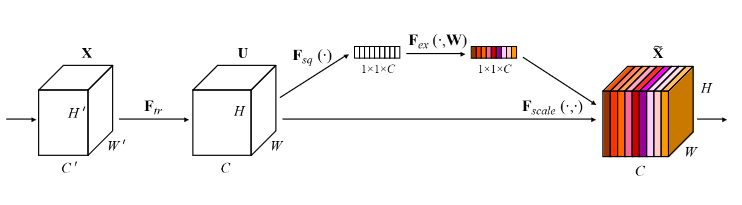
\includegraphics[scale=0.45]{src/BackgroundReading/assets/squeze_and_excitation.png}
    \caption{Squeeze-and-Excitation block architecture}\label{fig:squeze_and_excitation}
\end{figure*}

This type of CNN is a transitional link between classical CNN architecture 
and transformer architecture in CV~\cite{transformers}.
Authors of the paper\cite{seNet} propose a Squeeze-and-Excitation block that performs as 
attention mechanism that can be embedded in CNN architecture.

The main idea is to flatten each channel of the input feature map in a such way, 
that each channel would be represented by only one value. It can be done by
applying global average pooling to each channel:
\[F_{sq}(u_c) = z_c = \frac{1}{H\cdot W} \cdot \sum\limits_{i=1}^H\sum\limits_{j=1}^W u_c(i,j)\]
where $u_c$ \- input channel, $W$ and $H$ are spatial dimensions, $z_c$ \- result statistic

After that, it's needed to implement nonlinear interaction between channels, to do that
it's a good idea to use 2 fully connected layers, one with ReLU activation and the other
with simple sigmoid:
\[F_{ex}(z,W)=s = \sigma (W_2\cdot (\delta(W_1\cdot z)))\] 
where $z$ embeddings from previous step, $W_1 \in \mathbb{R}^{\frac{C}{r}\times C}$, 
$W_2 \in \mathbb{R}^{C \times \frac{C}{r}}$, $\sigma$ \- ReLU activation.

$r$ is a scale factor: fully connected layers are computationally heavy, so decreasing the
hidden layer is needed for optimization purposes.

Finally, $s$ should be scaled up to save spatial dimensions of input, to achieve this the input of the block can be multiplied on $s$ channel-wise:
\[F_{scale}(u_c)=\widetilde{x}_c = s_c \cdot u_c\]

The full architecture is shown in Figure~\ref{fig:squeze_and_excitation}.

This approach can be implemented in any architectures described above, it's 
computationally lightweight and gives a good accuracy boost ($1.7\% $ for MobileNet 
and $1.4\%$ for EfficientNet).

\subsubsection{General ideas}
Also important to mention, that all the described above approaches can't be 
implemented directly due to a lack of computational resources, so only its ideas 
will be taken. Such layers like batch normalisation\cite{batch_norm} or dropout\cite{dropout} also will be used,
because they prevent overfitting and let models converge faster, which is important,
due to the low size of the dataset.
